\documentclass[12pt]{extarticle}
\usepackage[utf8]{inputenc}
\usepackage{cite}
\usepackage{graphicx}
\usepackage{float}
\usepackage{amsmath}
\usepackage{hyperref}
\graphicspath{ {images/} }

\setlength{\parindent}{0pt}

\title{Experiments on Multi-Armed Bandit Problems}
\author{Ajay Subramanian}
\date{May 2019}

\begin{document}

\maketitle

\setcounter{secnumdepth}{0}

\section{Definition of the Problem}
The multi-armed bandit problem is a classic reinforcement learning example wherein pulling each arm of a slot machine returns us a stochastic reward $q_*(a)$, generated from an unknown probability distribution. Our objective is to identify the sequence of arms that achieves an optimality of some kind. This optimality condition can be defined in various ways, for instance, asymptotic correctness, regret, or PAC. There are some interesting observations that we can make about Bandit problems.

\begin{enumerate}
	\item Bandit problems are a subset of immediate RL problems in which we receive an undelayed reward $R_t$ for every action $a_t$ . Also, $R_t$ is a pure function of $a_t$ and independent of any state variables.
	\item A major challenge in solving such problems is handling the explore-exploit trade-off. More exploitation maximizes the obtained reward, but at the cost of identifying possible better arms. Excessive exploration can result in a more confident estimated reward $Q(a)$ but also increases the regret i.e. payoff lost out on while picking sub-optimal arms.
I have experimented and analyzed the $\epsilon$-Greedy, Softmax action selection, and UCB-1 algorithms on the 10-armed testbed described in \cite{Sutton1998}
\end{enumerate}

\section{Experiments}

\subsection{$\epsilon$-Greedy}

The $\epsilon$-Greedy algorithm leaves the explore-exploit decision to a hyperparameter $\epsilon$. Exploiting involves pulling the arm corresponding to the maximum value of $Q_t(a)$ while exploring involves pulling an arm, uniformly at random.

\begin{figure}[H]
	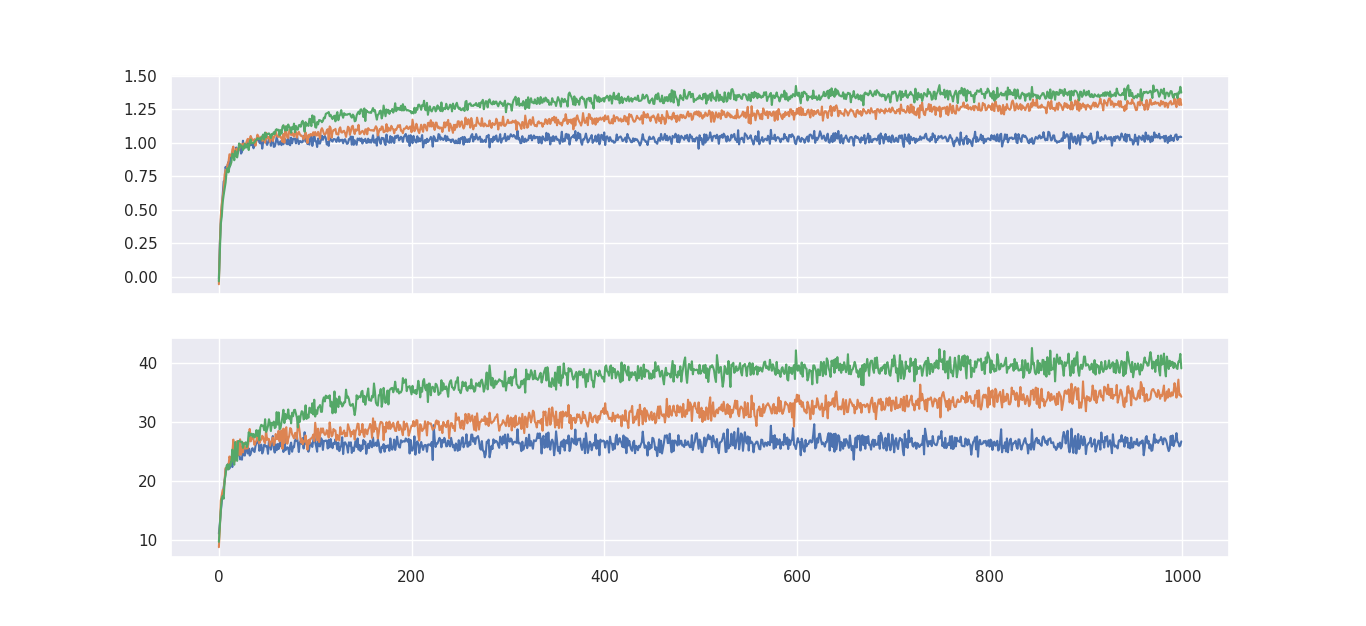
\includegraphics[width=\textwidth, height=10cm]{epsilon-greedy.png}
	\caption{reward vs time (top) and $\%$ optimal action vs time (bottom) for $\epsilon$-greedy for $\epsilon$ taking values 0 (blue), 0.01 (orange), 0.1 (green).}
	\label{fig:epsilon-greedy}
\end{figure}

As seen in first plot of Figure \ref{fig:epsilon-greedy}, when the algorithm is set to pure exploitation i.e. $\epsilon = 0$, the reward vs time plot sharply increases on the first trial and then stays almost constant throughout. This is because any arm that gives us a positive reward will become the only positive valued arm and hence the 'optimal' one. We will then continue pulling only that arm till the end of the process. This process of learning is entirely random and hence is not very reliable. Now, if $\epsilon$ is increased to $0.01$, we expect to take a random action $1\%$ of the time. Due to this, we see a sharp increase, followed by a gradual improvement in reward over time. The same trend holds for $\epsilon = 0.1$, but with the maximum possible reward being reached towards the final timesteps. This happens because, with a higher chance of exploration, it becomes easier to find the optimal arm. Hence, the average reward starts becoming more or less constant after timestep $\approx$750. Due to this 'reward saturation', we see the gap between the $\epsilon=0.01$ and $\epsilon=0.1$ curves decreasing towards the end.\\

This observation could also be explained from the perspective of explore-exploit tradeoffs. Whereas $\epsilon=0.1$ curve identifies the optimal arm faster and continues to randomize its actions even after that, the $\epsilon=0.01$ plot takes time to figure out the best arm, but almost always pulls that arm once it does.\\

The difference between these two $\epsilon$ values is all the more visible in the second plot of Figure \ref{fig:epsilon-greedy} where we see the best arm being learned by the $\epsilon=0.01$ model gradually over time while it is identified much earlier(at $\approx$400) by $\epsilon=0.1$.

\subsection{Softmax Action Selection}

Using a softmax action selection makes the probability of pulling each arm proportional to its estimated reward $Q_t(a)$. This makes the exploration process more efficient and helps us to eliminate the clearly undesirable arms.\\

\begin{figure}[H]
	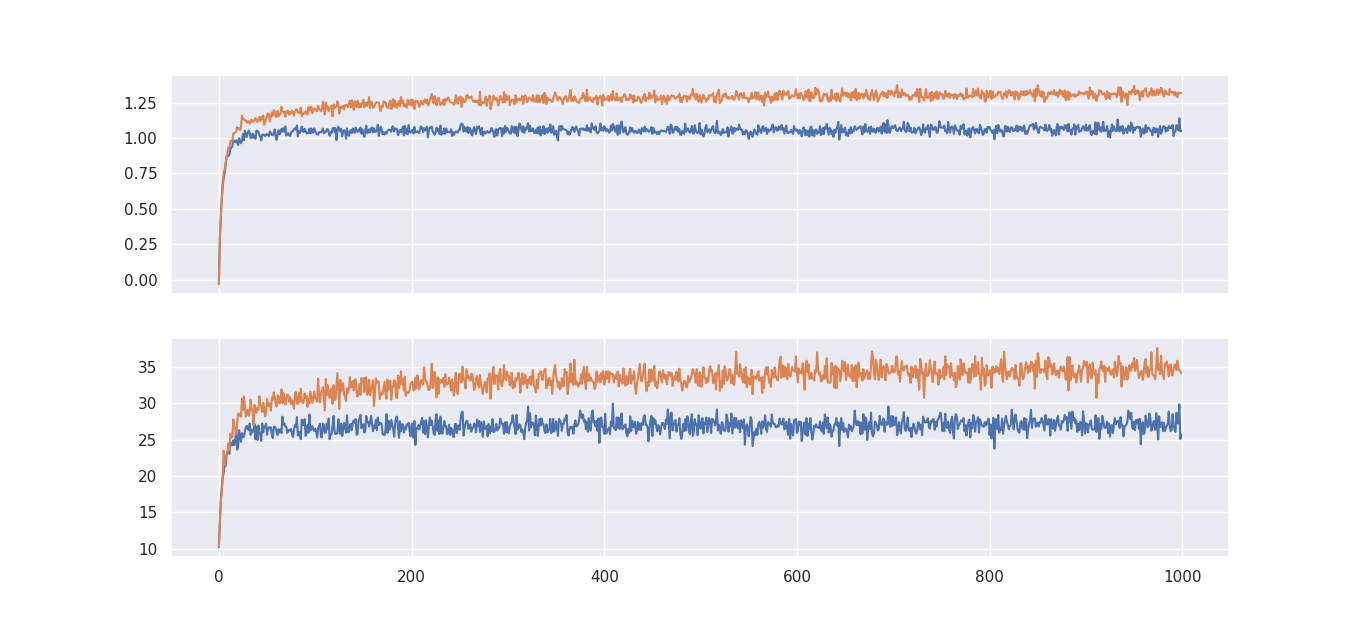
\includegraphics[width=\textwidth, height=10cm]{softmax-action-selection.png}
	\caption{reward vs time (top) and $\%$ optimal action vs time (bottom) for softmax action selection for $\beta$ taking values 0.01 (blue), 0.1 (orange)}
	\label{fig:softmax-action-selection}
\end{figure}

When we compare the curves in Figure \ref{fig:softmax-action-selection} with those in Figure \ref{fig:epsilon-greedy}, we can clearly make out that the maximization of reward occurs much earlier when we use softmax action selection. This is because of the more efficient action selection process. Arms that consistently return a lower reward will have a lower value function, and hence a lower probability of being selected. This is in contrast to the $\epsilon$-greedy case where exploring meant giving equal chances to each sub-optimal arm irrespective of how consistently badly or well they had performed in the past.\\

We would also like to observe the variation of the plots when the value of $\beta$ is changed, in this case for values 0.01 and 0.1. The most important difference is that a higher value of $\beta$ correlates to a more uniform probability distribution, and therefore more randomness in selection, while a lower $\beta$ value corresponds to a more biased distribution and hence more exploration.

\subsection{Upper Confidence Bound (UCB-1)}

While the two algorithms seen until now aim to achieve asymptotic correctness (choosing an arm that gives maximum payoff), the UCB-1 algorithm tries to, in addition, minimize regret i.e. pull least possible number of arms prior to finding the best one. Hence the algorithm goes as follows:

\begin{enumerate}
	\item \textbf{Pull each arm once:} This helps us get an early reward estimate of each arm. Asymptotically, pulling each arm atleast once is a necessity to make a decision about the optimum one.
	\item \textbf{Choose the arm j that maximizes $Q(j) + \sqrt{\frac{2\ln(n)}{n_j}}$:} UCB works on the principle of 'uncertain optimism'. This means that the algorithm hopes for an arm better than what is observed from previous data. This is clear in the above expression where the second term can be understood as an exploration confidence interval which shrinks as we pull more arms. This happens since as we pull more arms, we become more confident about the estimated reward values.
\end{enumerate}

\begin{figure}[H]
	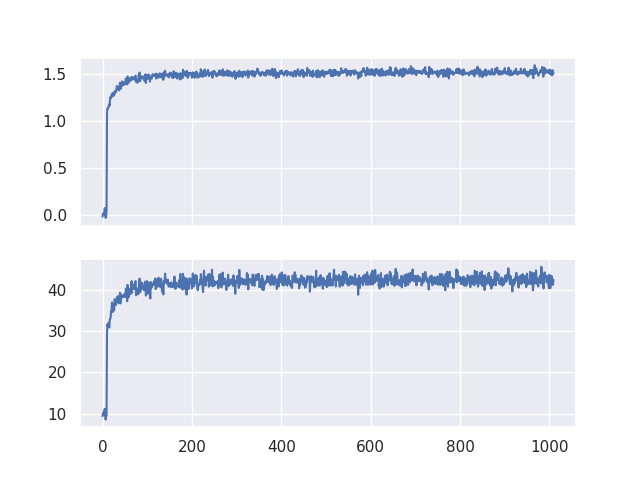
\includegraphics[width=\textwidth, height=10cm]{ucb-1.png}
	\caption{reward vs time (top) and $\%$ optimal action vs time (bottom) for UCB-1}
	\label{fig:ucb-1}
\end{figure}

It is easily observable from Figure \ref{fig:ucb-1} that UCB-1 achieves the near-optimum action the fastest amongst the three algorithms. An important reason for this is that UCB, unlike $\epsilon$-greedy and softmax, combines the explore and exploit phases into a single operation. This is explained as follows. We have already seen the following action selection metric.\\

\begin{equation*}
argmax_j \left(Q(j) + \sqrt{\frac{2\ln(n)}{n_j}}\right)
\end{equation*}

The first term of the expression accounts for exploitation. We know that, in order to maximize our reward and minimize the regret, we have to take an action with a reward somewhere in the vicinity of the known optimum. Next, at each step, we try to explore in the region by aiming for a slightly higher reward. The second term accounts for this exploration effort. Hence, due to each step of UCB being productive, we can expect it to learn much faster than both $\epsilon$-greedy and softmax, both of which need more time due to separate explore and exploit phases.\\

\section{Effect of a Larger Action Space \footnote{Graphs corresponding to this section can be accessed \href{https://github.com/ajaysub110/RL-experiments/tree/master/bandit/viz}{here}}}
The major difference in these three algorithms is action selection i.e. the method of deciding and optimizing the explore-exploit decision. However, in the big picture, they work towards a common objective that is arriving at a good estimation for the true reward distribution. This distribution becomes harder to estimate, as the number of arms increases since the agent is left with more options per decision. Therefore all three algorithms share the characteristic that they take more timesteps to figure out the optimal action, as the number of arms increases.There are however, a few differences in the trend followed by each algorithm

\subsection{$\epsilon$-Greedy}

As the number of arms increases, the trained bandits perform much better (on average) than the case with fewer arms, though they take longer to get trained. This could be because having more arms (with values picked from a common distribution) results in a lower probability of a few bad arms being picked. But in the few arms case, one bad arm could easily be picked since the sample size is much smaller.

\subsection{Softmax}
The effect discussed above is prevalent in softmax too. But since the softmax distribution biases us towards picking a better arm even in the few-arms case, the effect of more arms is not as pronounced.

\subsection{UCB-1}
The trend seen in the UCB case is quite different from the other algorithms. In the first 1000 (number of arms) timesteps, it averages a reward of 0 because UCB initially picks each arm once. After that, it starts pulling arms with an optimistic reward expectation. But in a more-arms case, the algorithm behaves more aggressively because at initial timesteps, the $\frac{2\ln(n)}{n_j}$ value is smaller. Due to this, the increase in reward is slower but for more significant over a large number of timesteps.\\
Another interesting observation in the UCB graph is that it has a higher optimal action percentage than the other algorithms. This could be because of the simultaneous exploration-exploitation by UCB i.e taking random actions from an estimated confidence interval rather from the whole action space.

\section{REINFORCE on Contextual Bandits}
\begin{figure}[H]
	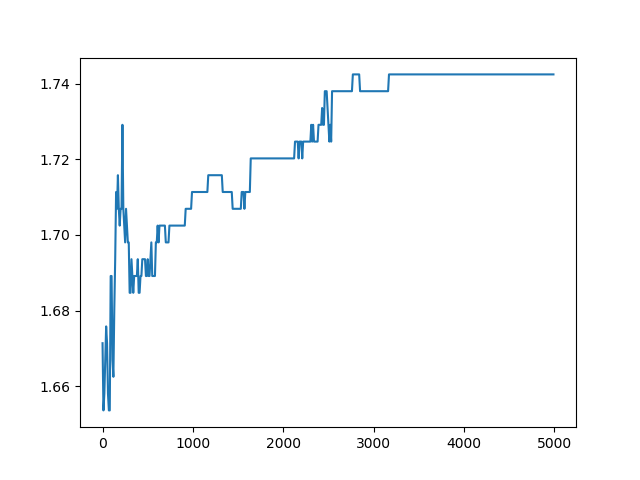
\includegraphics[width=\textwidth, height=10cm]{reinforce.png}
	\caption{reward vs time for REINFORCE on a Contextual Bandit problem}
	\label{fig:reinforce}
\end{figure}
 
A contextual bandit problem is a problem that is modelled using different bandits (different distributions) for different states. When encountered with a particular state, we pick an action corresponding to our estimation of the expected reward of only that bandit (state). Contextual bandits are an acceptable formulation when we have states that are independent of each other i.e which is a more extreme assumption than the Markov assumption, and not always true in real world environments.\\
REINFORCE works by ascending the gradient of the estimated reward function. However, it may encounter local maxima or saddle points in its journey to the global maximum. Hence, the reward vs time graph as seen in Figure \ref{fig:reinforce} may not always be a monotonically increasing graph (unlike the algorithms seen so far).
The speed of convergence is determined by the step size. Too small a step size makes it slow while a very large one might result in an oscillation in the reward function.\\
An advantage of REINFORCE (or any policy gradient method) is that they can be modelled using a MLP, whence a sequence of linear operations with non-linear activation functions can result in complex function approximation capabilities.\\

\section{Conclusion}
From the detailed analyses of three perspectives at solving bandit problems, we have now a better understanding of the deep intuitions involved in their design. We have also analyzed the role of parameters in the functioning of these algorithms and have learnt the expected behavior of these models with varying parameter values.\\

\bibliography{cites}
\bibliographystyle{ieeetr}

\end{document}